%%%%%%%%%%%%%%%%%%%%%%%%%%%%%%%%%%%%%%%%%%%%%%%%%%%%%%%%%%%%%%%%%%%%%%%%%%%%%%%
\chapter{Additional Information about the Dataset}
\label{ch:appendix2:dataset}
%%%%%%%%%%%%%%%%%%%%%%%%%%%%%%%%%%%%%%%%%%%%%%%%%%%%%%%%%%%%%%%%%%%%%%%%%%%%%%%

\begin{figure}[htb]
	\centering
	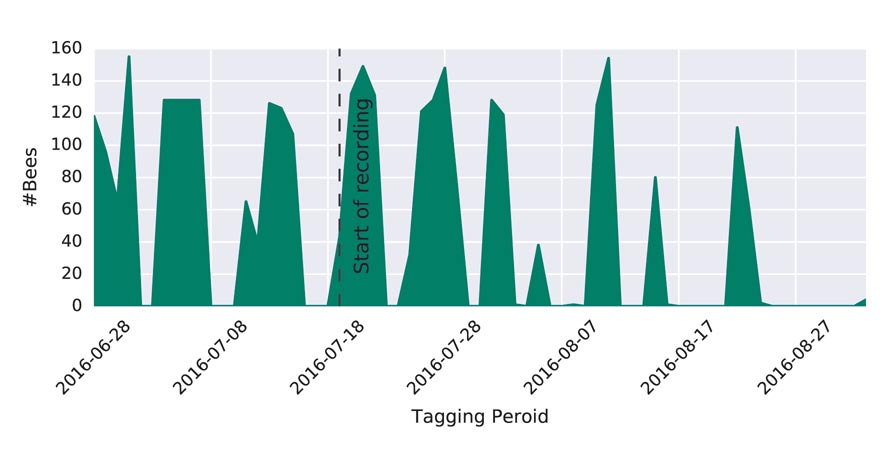
\includegraphics[width=1.0\textwidth]{Figures/tagging_period}
	\caption[Tagging frequency]{\textbf{Tagging frequency} The bees were primarily tagged during the week. On average 48 bees were tagged each day, considering only tagging days, the average is about 91.}
	\label{fig:tagging-period}
\end{figure}

\begin{figure}[htb]
	\centering
	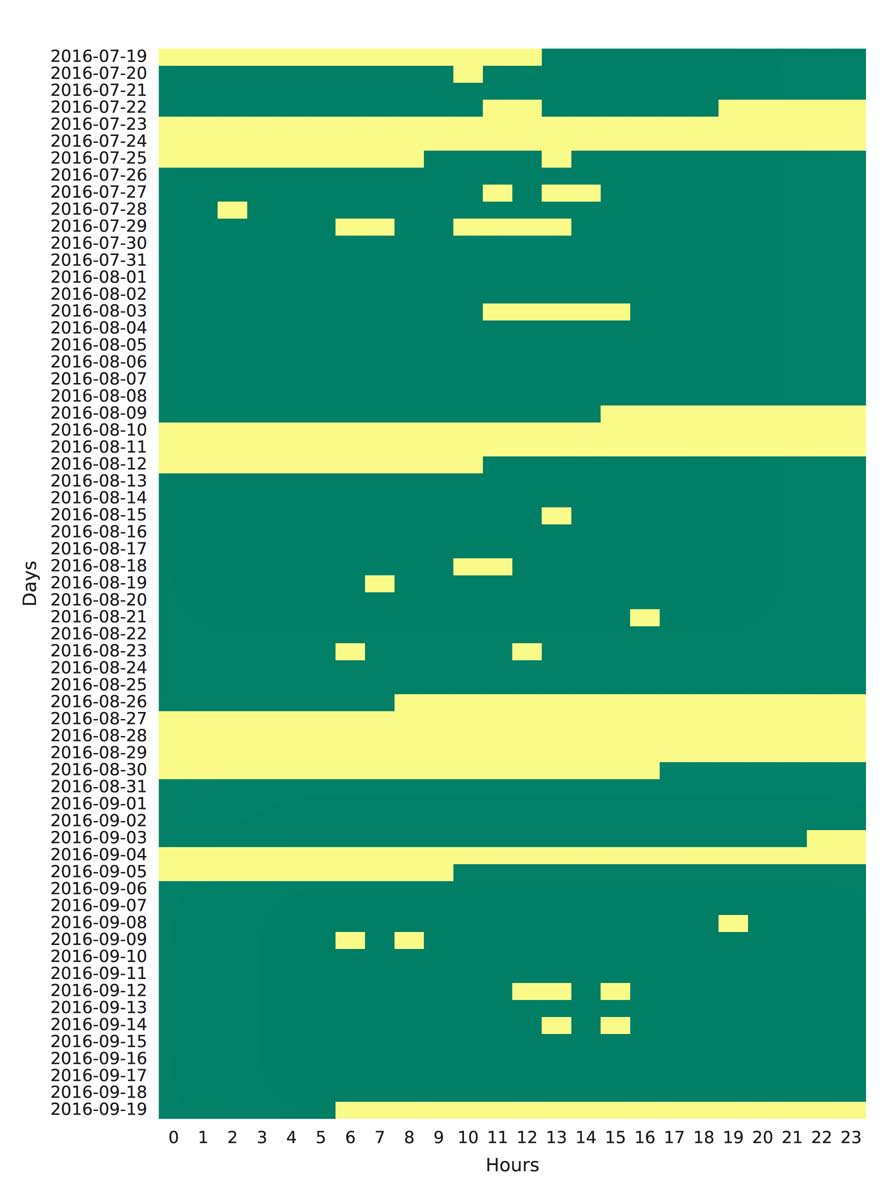
\includegraphics[width=1.0\textwidth]{Figures/recording}
	\caption[Recording season with maintainance and failures]{\textbf{Recording season with maintainance and failures} \emph{Green} indicates recording went without any big interruption; \emph{Yellow} indicates maintainance work or technical failures of one or all cameras. This is calculated using the expected number of files produced by each camera per hour.}
	\label{fig:observation-period}
\end{figure}